\usepackage{hyperref}
\usepackage{graphicx}
\usepackage{listings}
\usepackage{textcomp}
\usepackage{fancyvrb}

\title{Ethics in Software Development: Time Traveler Edition}
\subtitle{Back...from the future}
\author{Moshe Zadka -- https://cobordism.com}
\date{2019}

\begin{document}
\begin{titlepage}
\maketitle
\end{titlepage}

\frame{\titlepage}

\begin{frame}[fragile]
\frametitle{Who am I}

\begin{itemize}
\item Born: July 10th, 2258
\item Certified Software Developer (passed exams Jan 22nd, 2287)
\item No formal higher education
\end{itemize}

\end{frame}

I have to let you all in on a little secret.
I was born in the future.
2258, to be precise.
Until I travelled back in time,
I was working as a certified software developer ever since
I passed my exams in 2287.

I don't want to go into the details of my time travel.
I want to talk about the differences in software development.
I want to talk about software developer ethics.
A code of ethics.
But what is a code of ethics?


\begin{frame}[fragile]
\frametitle{Ethic codes are trolleys}

\begin{figure}
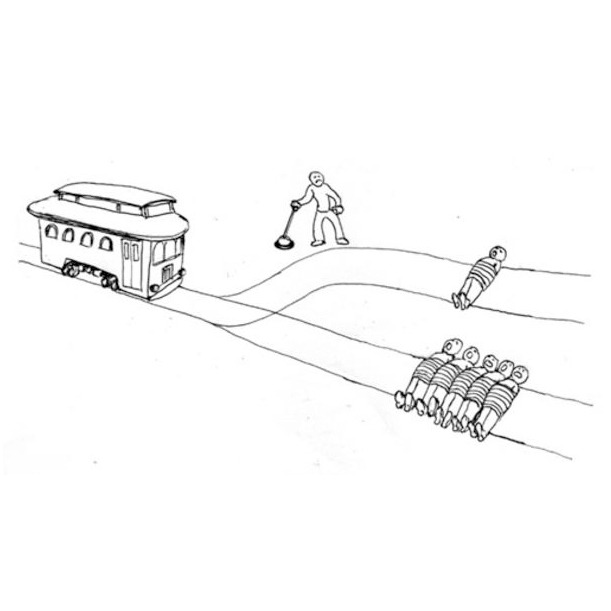
\includegraphics[scale=0.25]{trolley}
\end{figure}

\end{frame}

Ultimately, a code of ethics consists of
"solutions"
to trolley problems:
a case where,
regardless of what we do,
some damage will be done.
A code of ethics tells us who to damage.
In the most of extreme of cases,
a code of ethics tells us who to kill.

So why do we want a code of ethics?
Why do we want to kill?
It is because in some professions,
you are going to be responsible for the life of people.
This responsibility for life is part of what you get
when you choose the profession.
This is something even you 21st century folks know:
some professions have accepted that part of their responsibilities
is making life and death decisions.

\begin{frame}[fragile]
\frametitle{Ethics in 21st century: civil engineers}

\begin{itemize}
\item Example: Act as faithful agent\pause
\item Example: Issue true statement\pause
\item Example: Service with competence
\end{itemize}

\end{frame}

Close to software developers,
civil engineers is also a profession where a lot of technical knowledge
and understanding of abstract principles is used to create
things people use every day.
Since they have been building things since the dawn of time,
and occasionally those collapse killing thousands,
civil engineers had to already think about what their ethics should look like.

\begin{frame}[fragile]
\frametitle{Ethics in 21st century: lawyers}

\begin{itemize}
\item Example: Confidentiality of information\pause
\item Example: Competence\pause
\item Example: No counsel to criminal actions
\end{itemize}

\end{frame}

Lawyers,
as welll,
have their code of ethics.
Part of their job is dealing with people who broke the law,
or possibly broke the law,
or who plan to have very interesting relationships with the law.
Regardless of whether the law is just or not,
a lawyer is not allowed to give advice to violate the law.
Regardless of how bad the secrets confided in them,
a lawyer cannot divulge them.

\begin{frame}[fragile]
\frametitle{Ethics in 21st century: doctors}

\begin{itemize}
\item Example: Responsibility to patient is paramount\pause
\item Example: Commitment to medical education\pause
\item Example: Report physicians engaging in fraud
\end{itemize}

\end{frame}

Another profession who can see their responsibility
for life and death,
since they deal,
often,
with bodies that are near death,
is doctors.
They have their own unique code of ethics,
that is applicable for their constraints.

However,
in the 21st century,
we have no widely accepted code of ethics.
The ACM has a code that has none of the rigor
that the other codes have,
and with none of the training that back them.
Of course,
the other thing the ACM code lacks is enforcement.
Doctors who violate ethics cannot practice medicine.
Lawyers cannot practice law.
There are no consequences for software developers.


\begin{frame}[fragile]
\frametitle{The Incident}

\begin{figure}
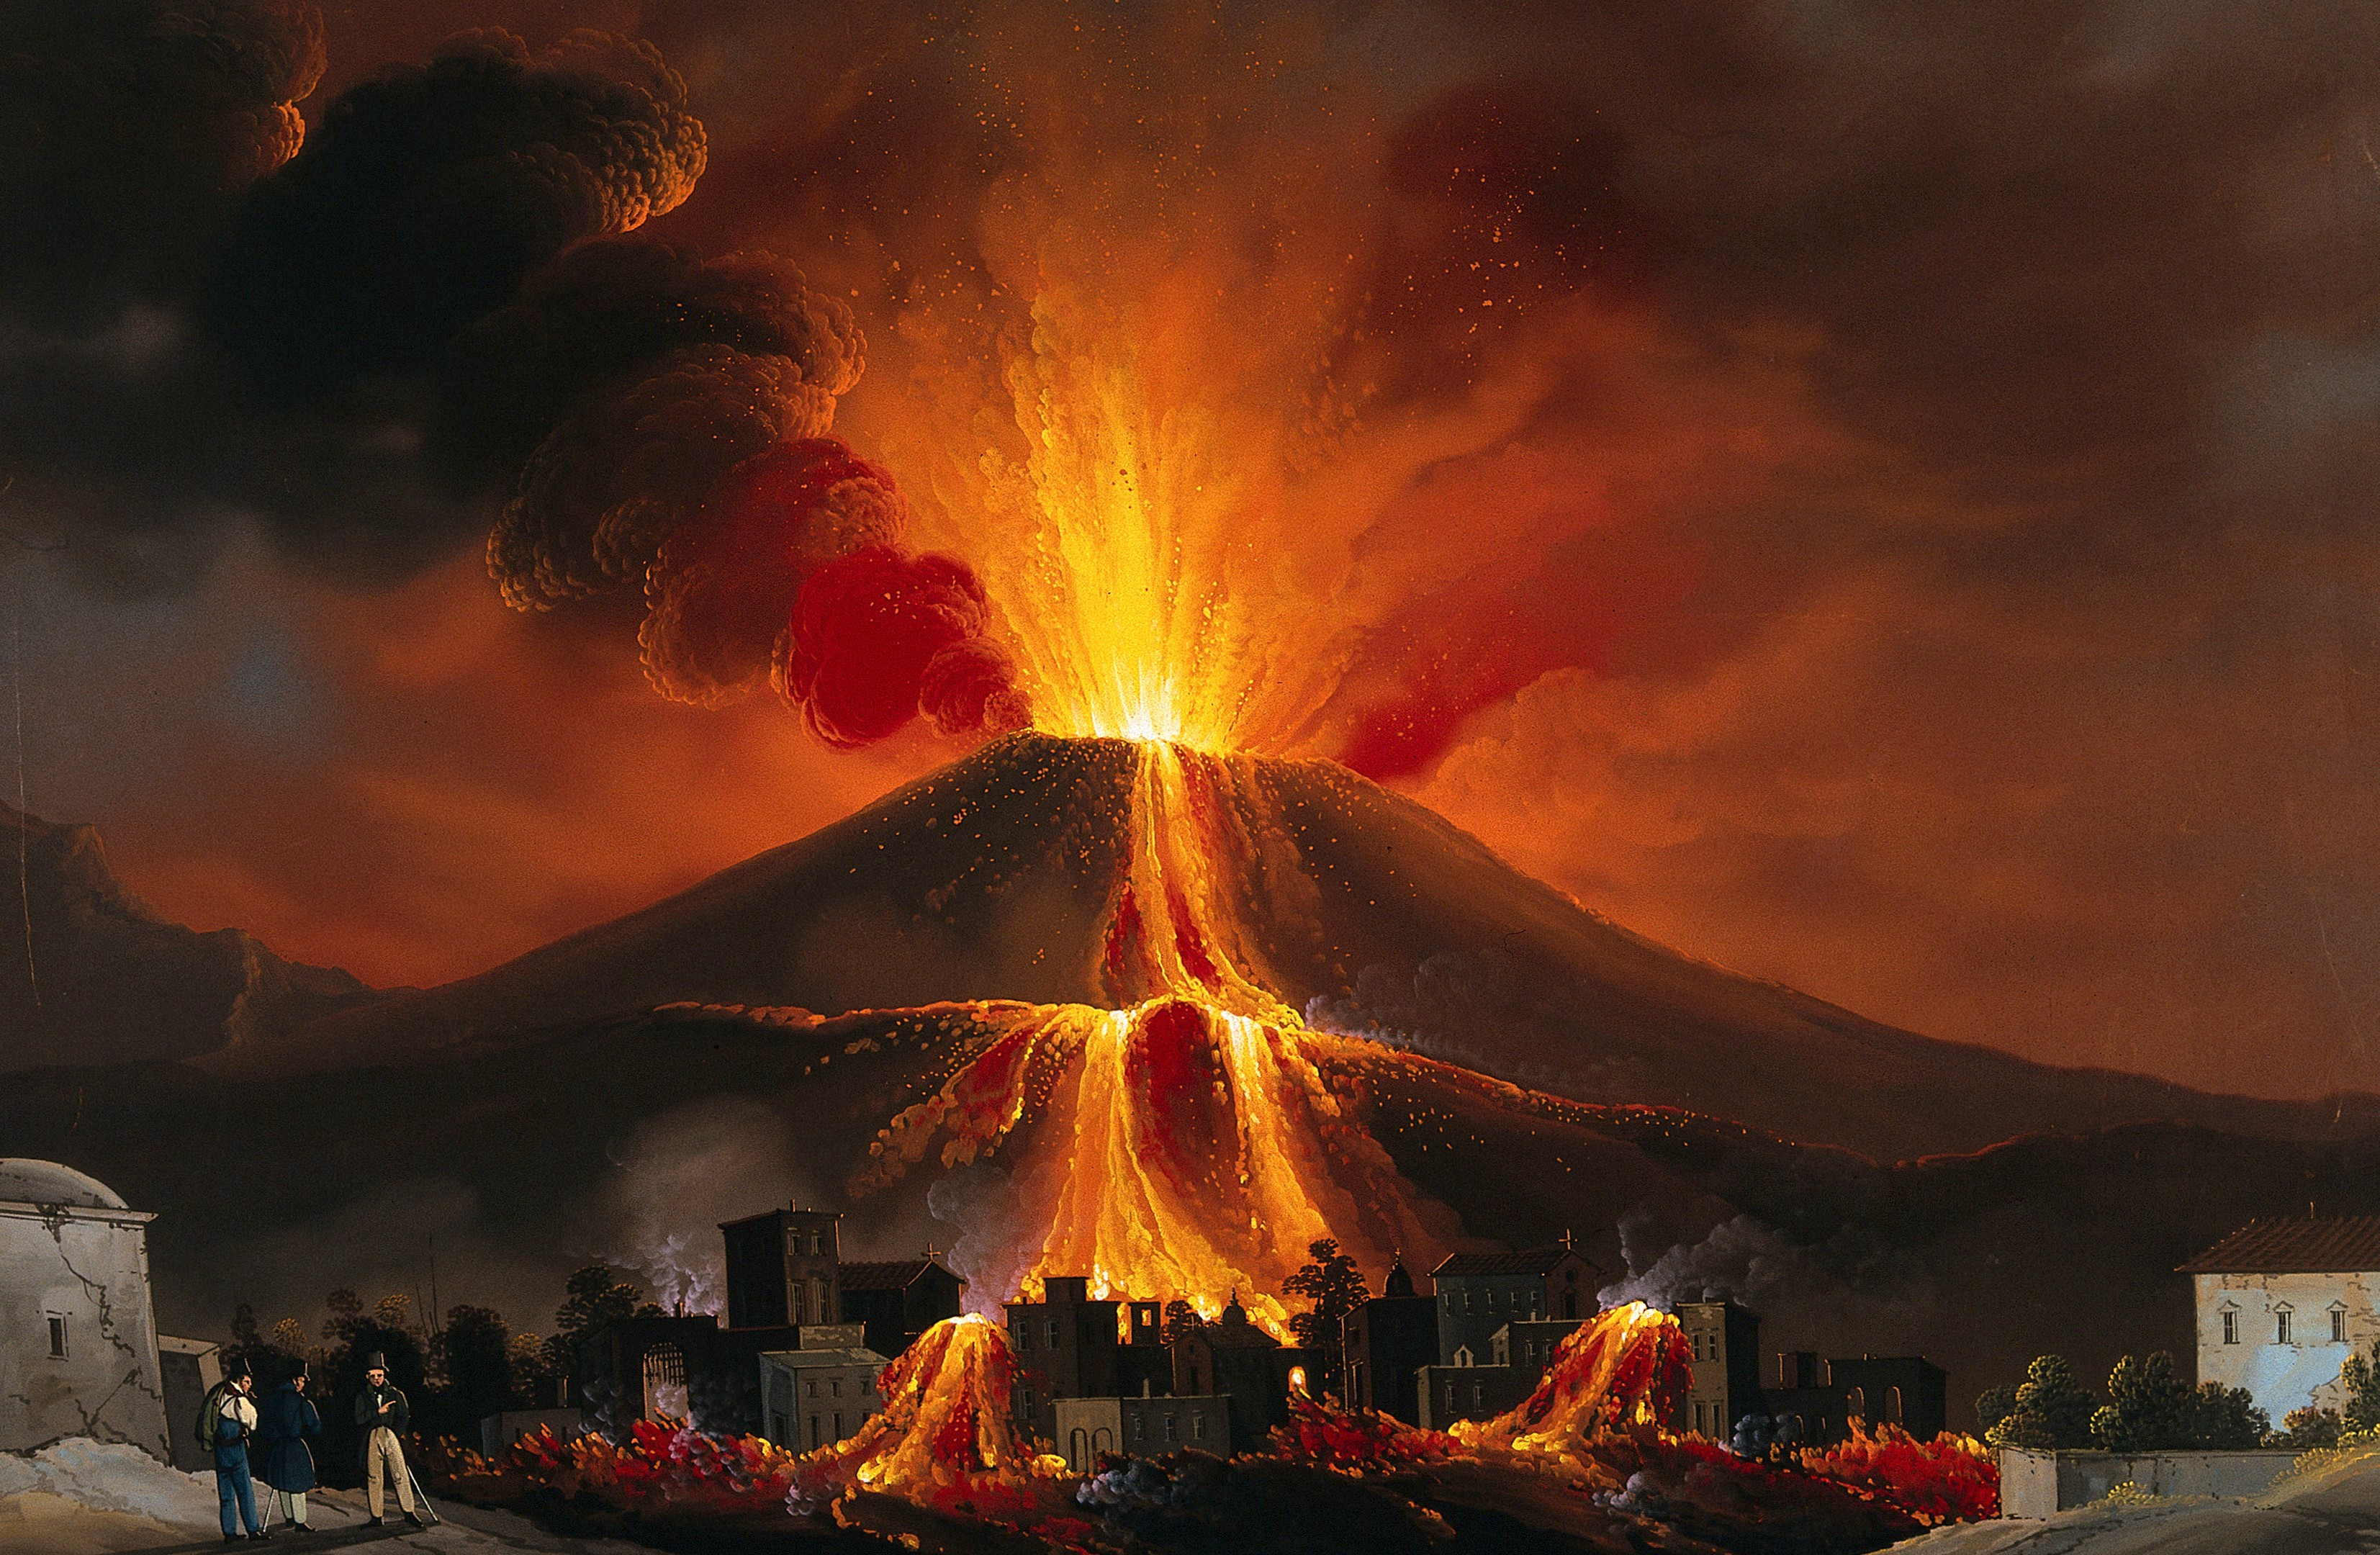
\includegraphics[scale=0.1]{volcano}
\end{figure}

\end{frame}

This,
in part,
is what led to the incident.
We do not like to talk about the incident.
I am not going to talk about it.
I'll just mention,
it was bad.
Really bad.
And there was no doubt that this was a direct cause
of software development being completely unregulated.

\begin{frame}[fragile]
\frametitle{The Incident: Causes}

\begin{figure}
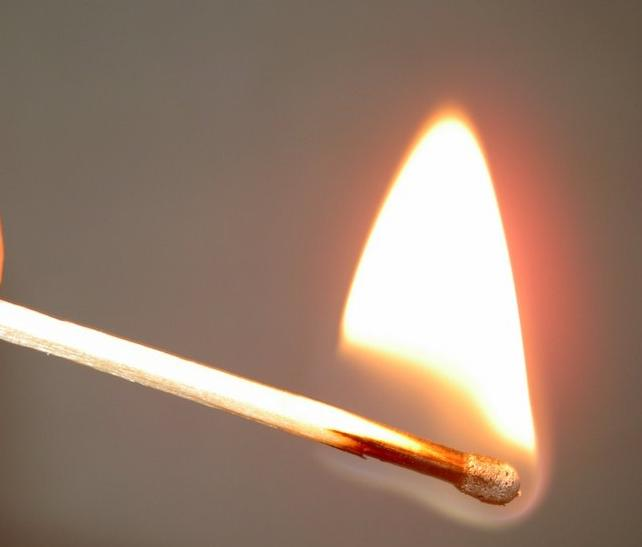
\includegraphics[scale=0.5]{match}
\end{figure}

\end{frame}


\begin{itemize}
\item Accountability?
\item User expectations
\item Big picture?
\end{itemize}

\begin{frame}[fragile]
\frametitle{The Incident: Consequences}

\begin{figure}
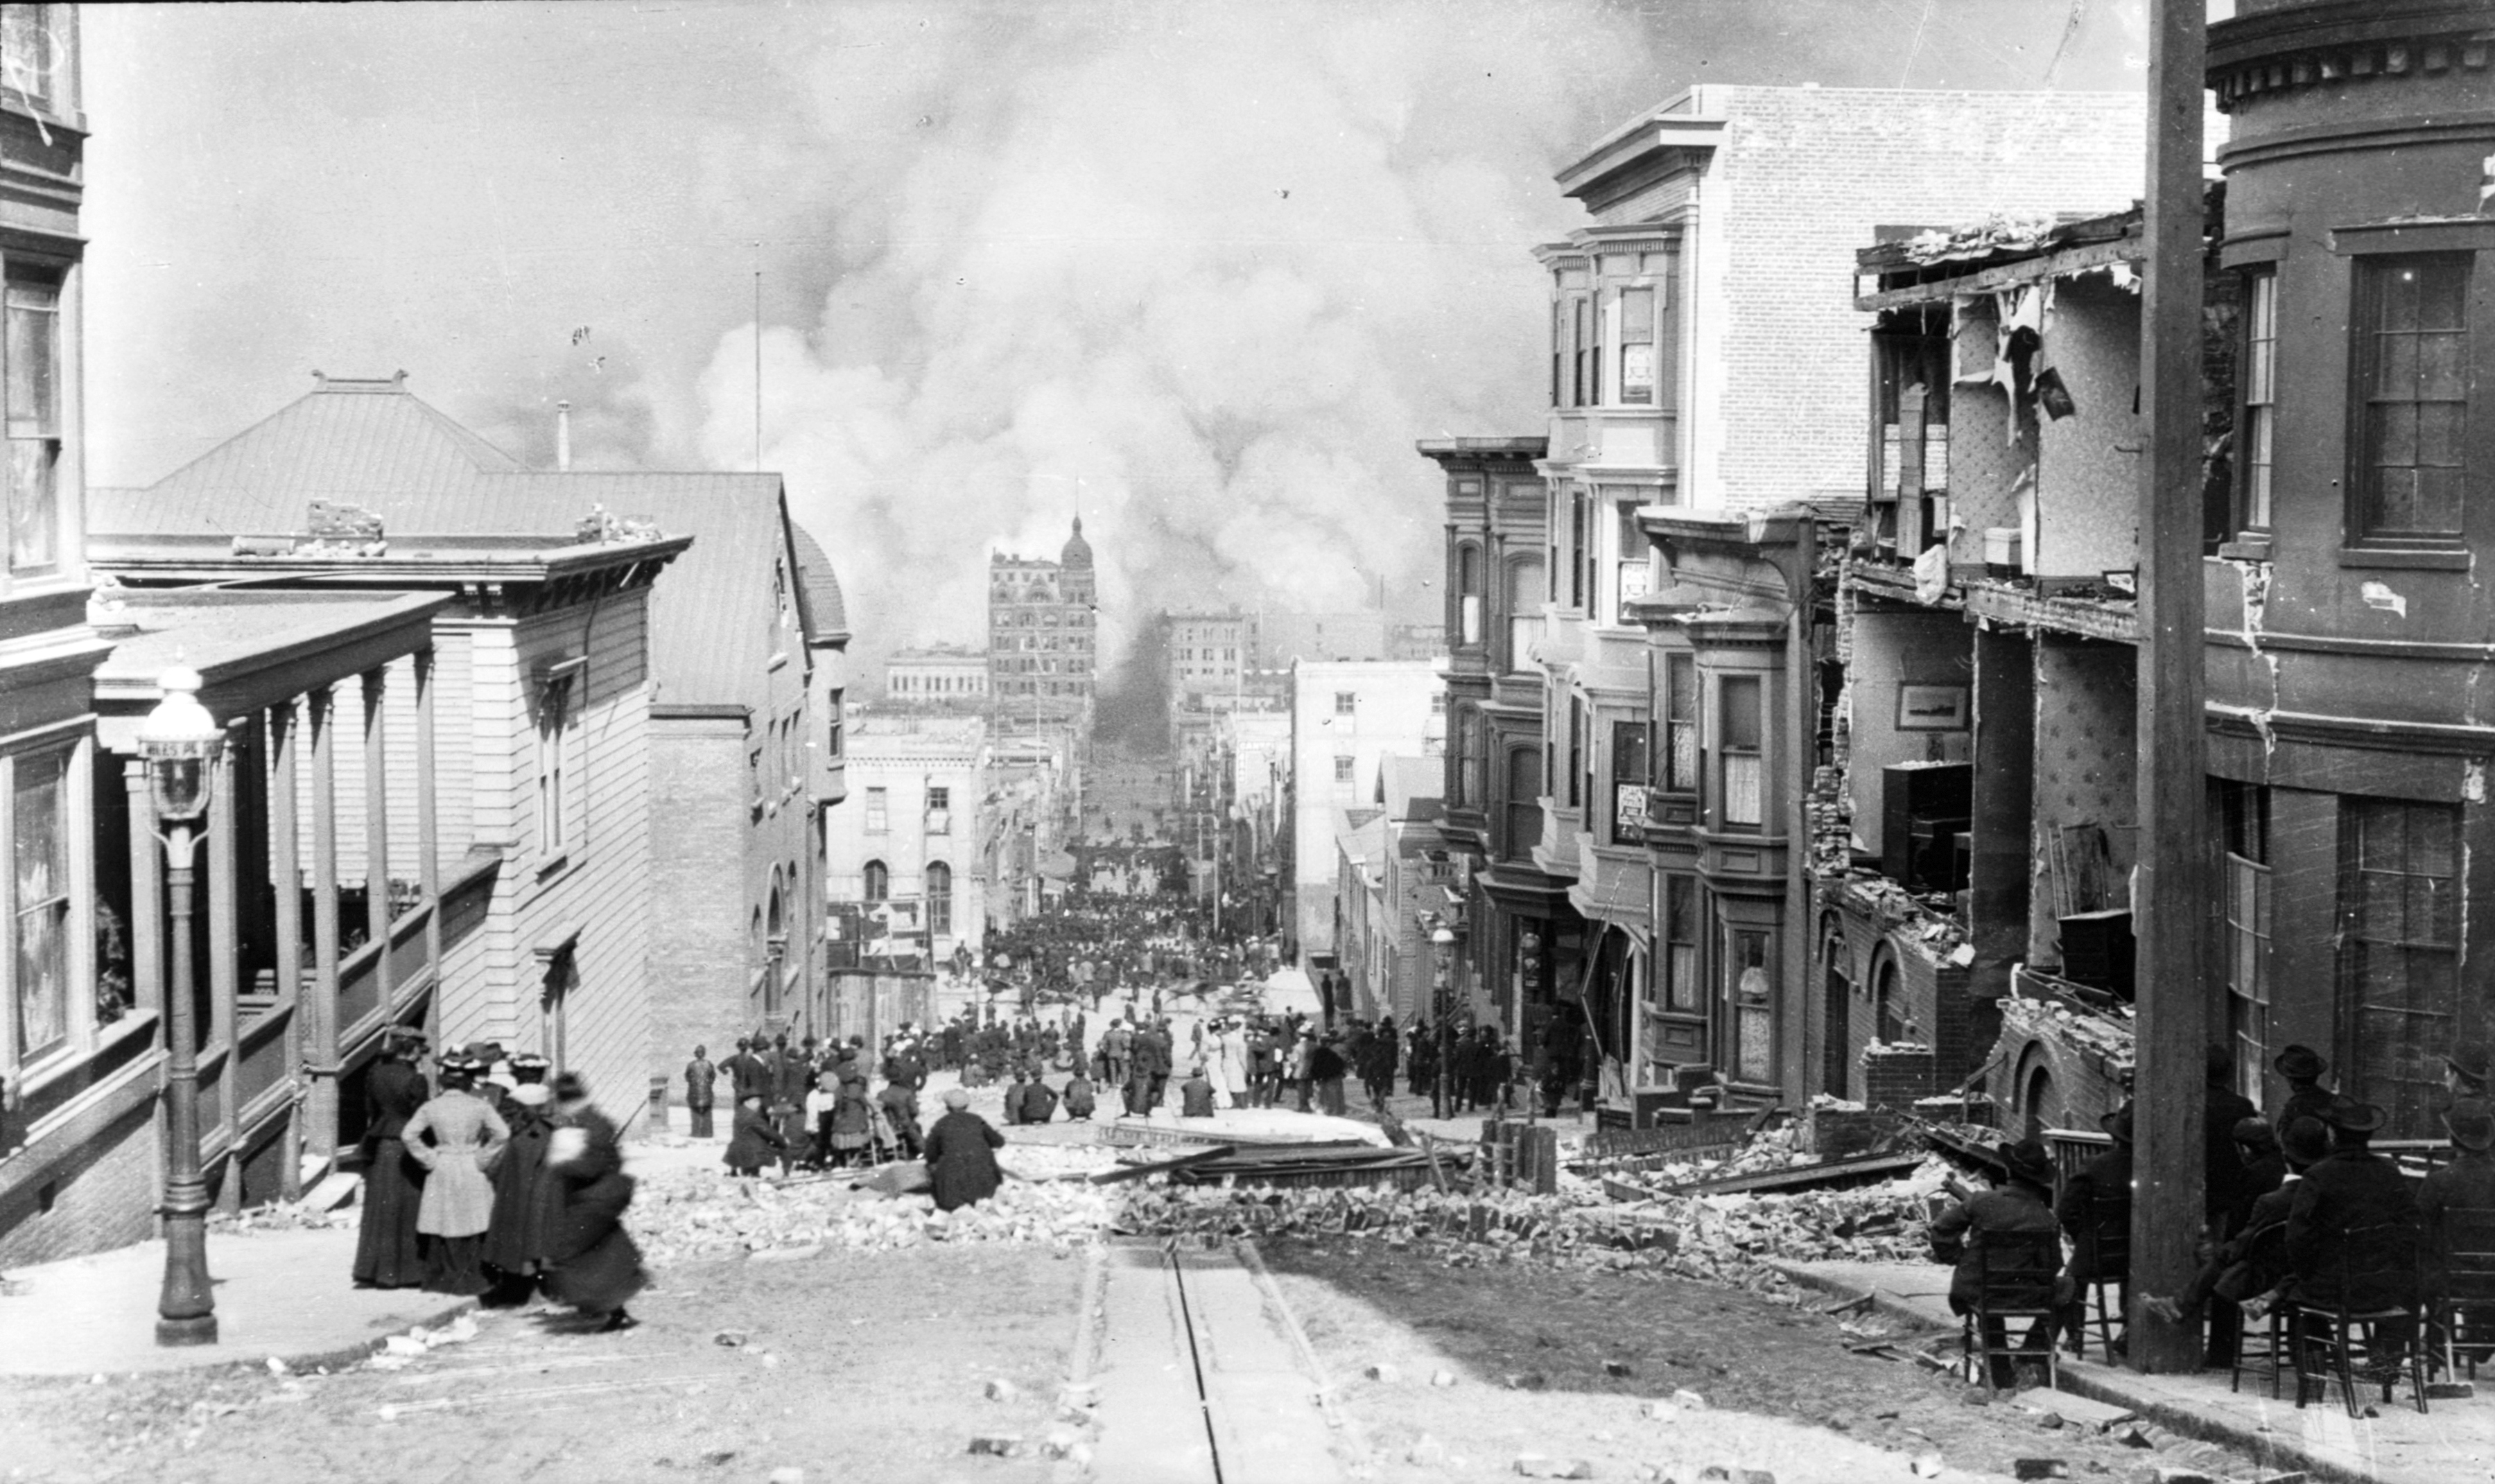
\includegraphics[scale=0.5]{fire}
\end{figure}

\end{frame}


\begin{itemize}
\item Billions of dollars' worth destroyed
\item Signifcant death toll
\item Businesses bankrupt
\end{itemize}

\begin{frame}[fragile]
\frametitle{The Incident: Aftermath}

\begin{figure}
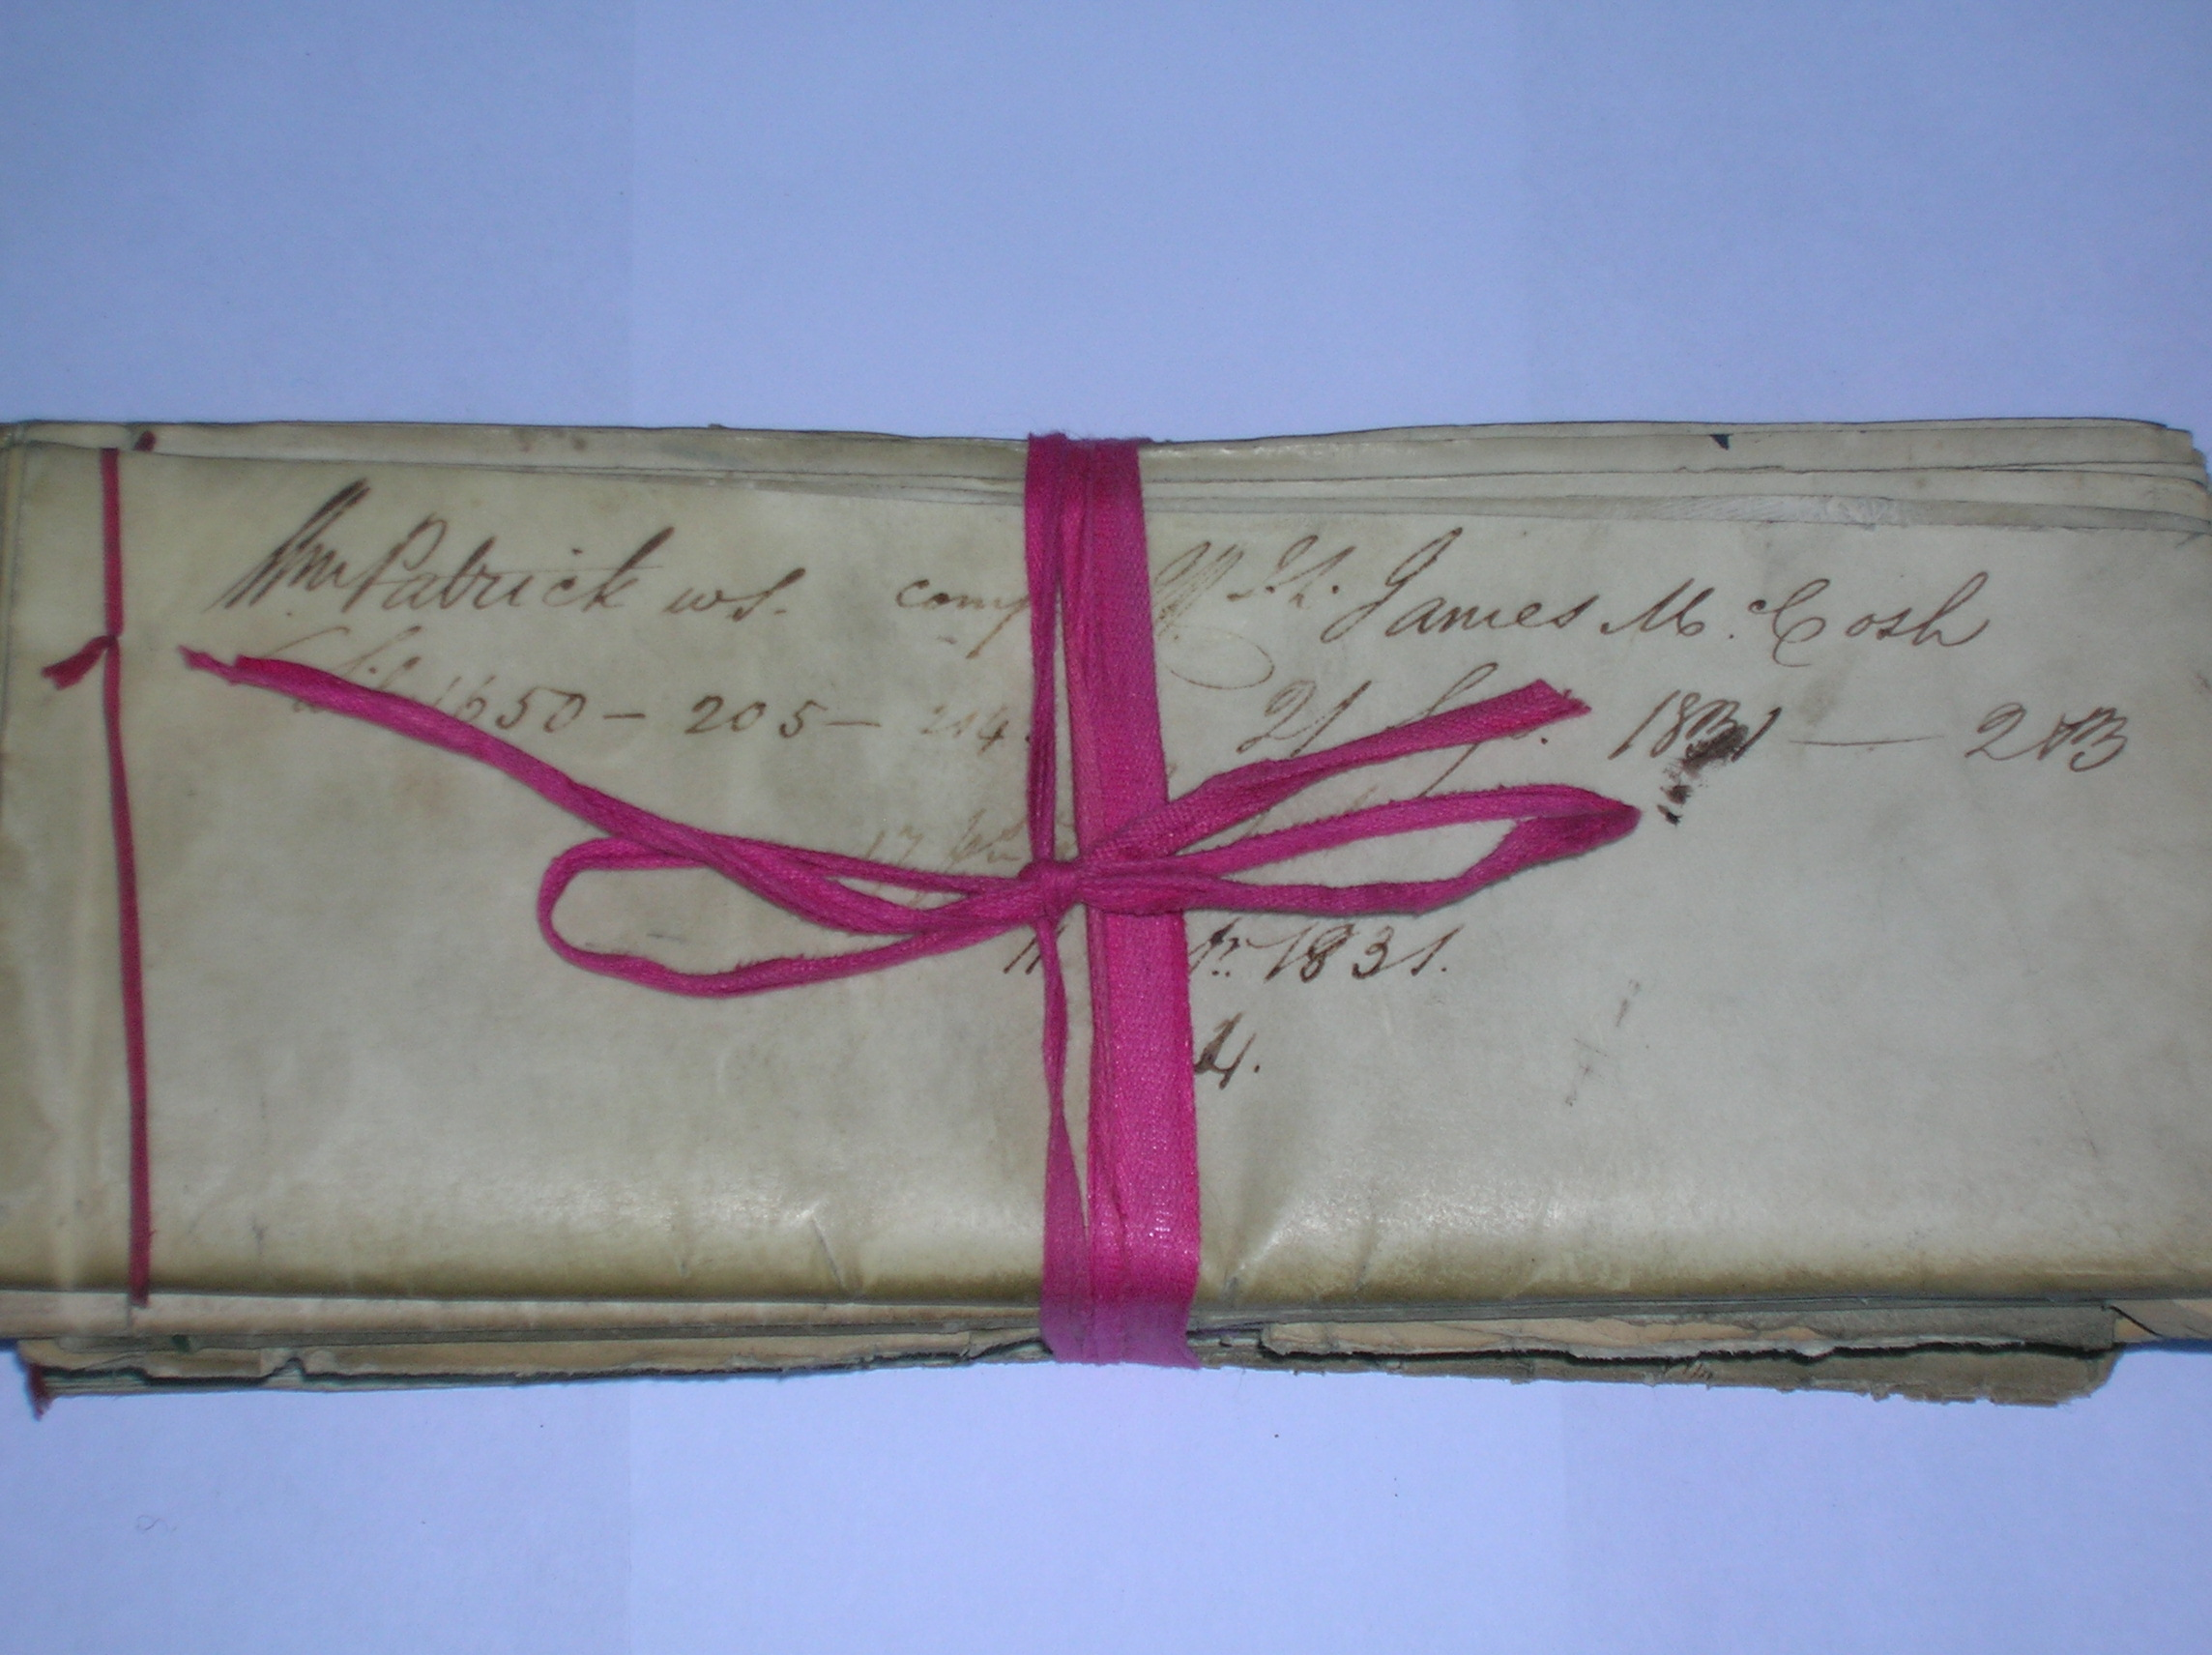
\includegraphics[scale=0.5]{redtape}
\end{figure}

\end{frame}

Redtape: \verb|https://commons.wikimedia.org/wiki/File:Redtape1.JPG|

\begin{itemize}
\item Regulation!
\item What makes software "fit for use"?
\item Who can write software?
\end{itemize}?

\begin{frame}[fragile]
\frametitle{23rd century}

It took a while...

\end{frame}

\begin{frame}[fragile]
\frametitle{OS Updates}

\begin{itemize}
\item Signed
\item Mandatory
\end{itemize}

\end{frame}

\begin{frame}[fragile]
\frametitle{Application stores}


\begin{figure}

\includegraphics{google_badge}
\end{figure}
\begin{figure}

\includegraphics[scale=0.15]{microsoft_badge}
\end{figure}


\end{frame}

\begin{itemize}
\item Competition
\item Bonded accountability
\item 5 "general purpose"
\item 20-30 "special purpose" (porn, kid entertainment)
\item Certificate authorities
\end{itemize}

\begin{frame}[fragile]
\frametitle{Publishing on application stores}

Software Development Studio is a legal category

\end{frame}

\begin{itemize}
\item Government registration
\item Certified software developers
\item Publish to application stores
\end{itemize}

\begin{frame}[fragile]
\frametitle{Certified software developers}


\begin{figure}
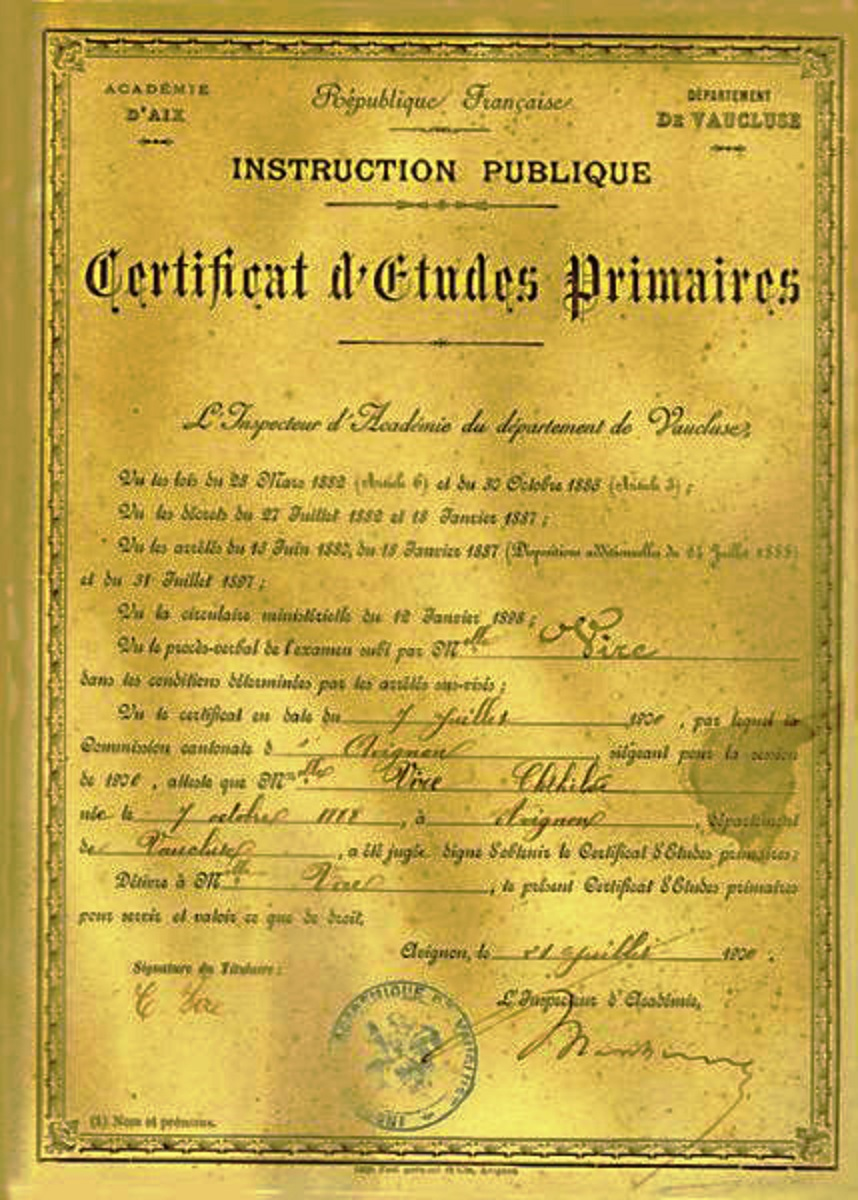
\includegraphics[scale=0.2]{certificate}
\end{figure}

\end{frame}

certificate: \verb|https://commons.wikimedia.org/wiki/File:1901_Certificat_d%27%C3%A9tudes_primaires.jpg|

\begin{itemize}
\item Pass the bar
\item Take an oath
\item Can be revoked
\end{itemize}

\begin{frame}[fragile]
\frametitle{Hobbyist coding}

\begin{figure}
\includegraphics[scale=0.05]{sandbox}
\end{figure}

\end{frame}

sandbox: \verb|https://upload.wikimedia.org/wikipedia/commons/a/a1/Sandkasse_sand_box_Norway.jpg|

\begin{itemize}
\item Developer mode
\item Sandbox
\end{itemize}



\begin{frame}[fragile]
\frametitle{Privacy laws}

\begin{figure}
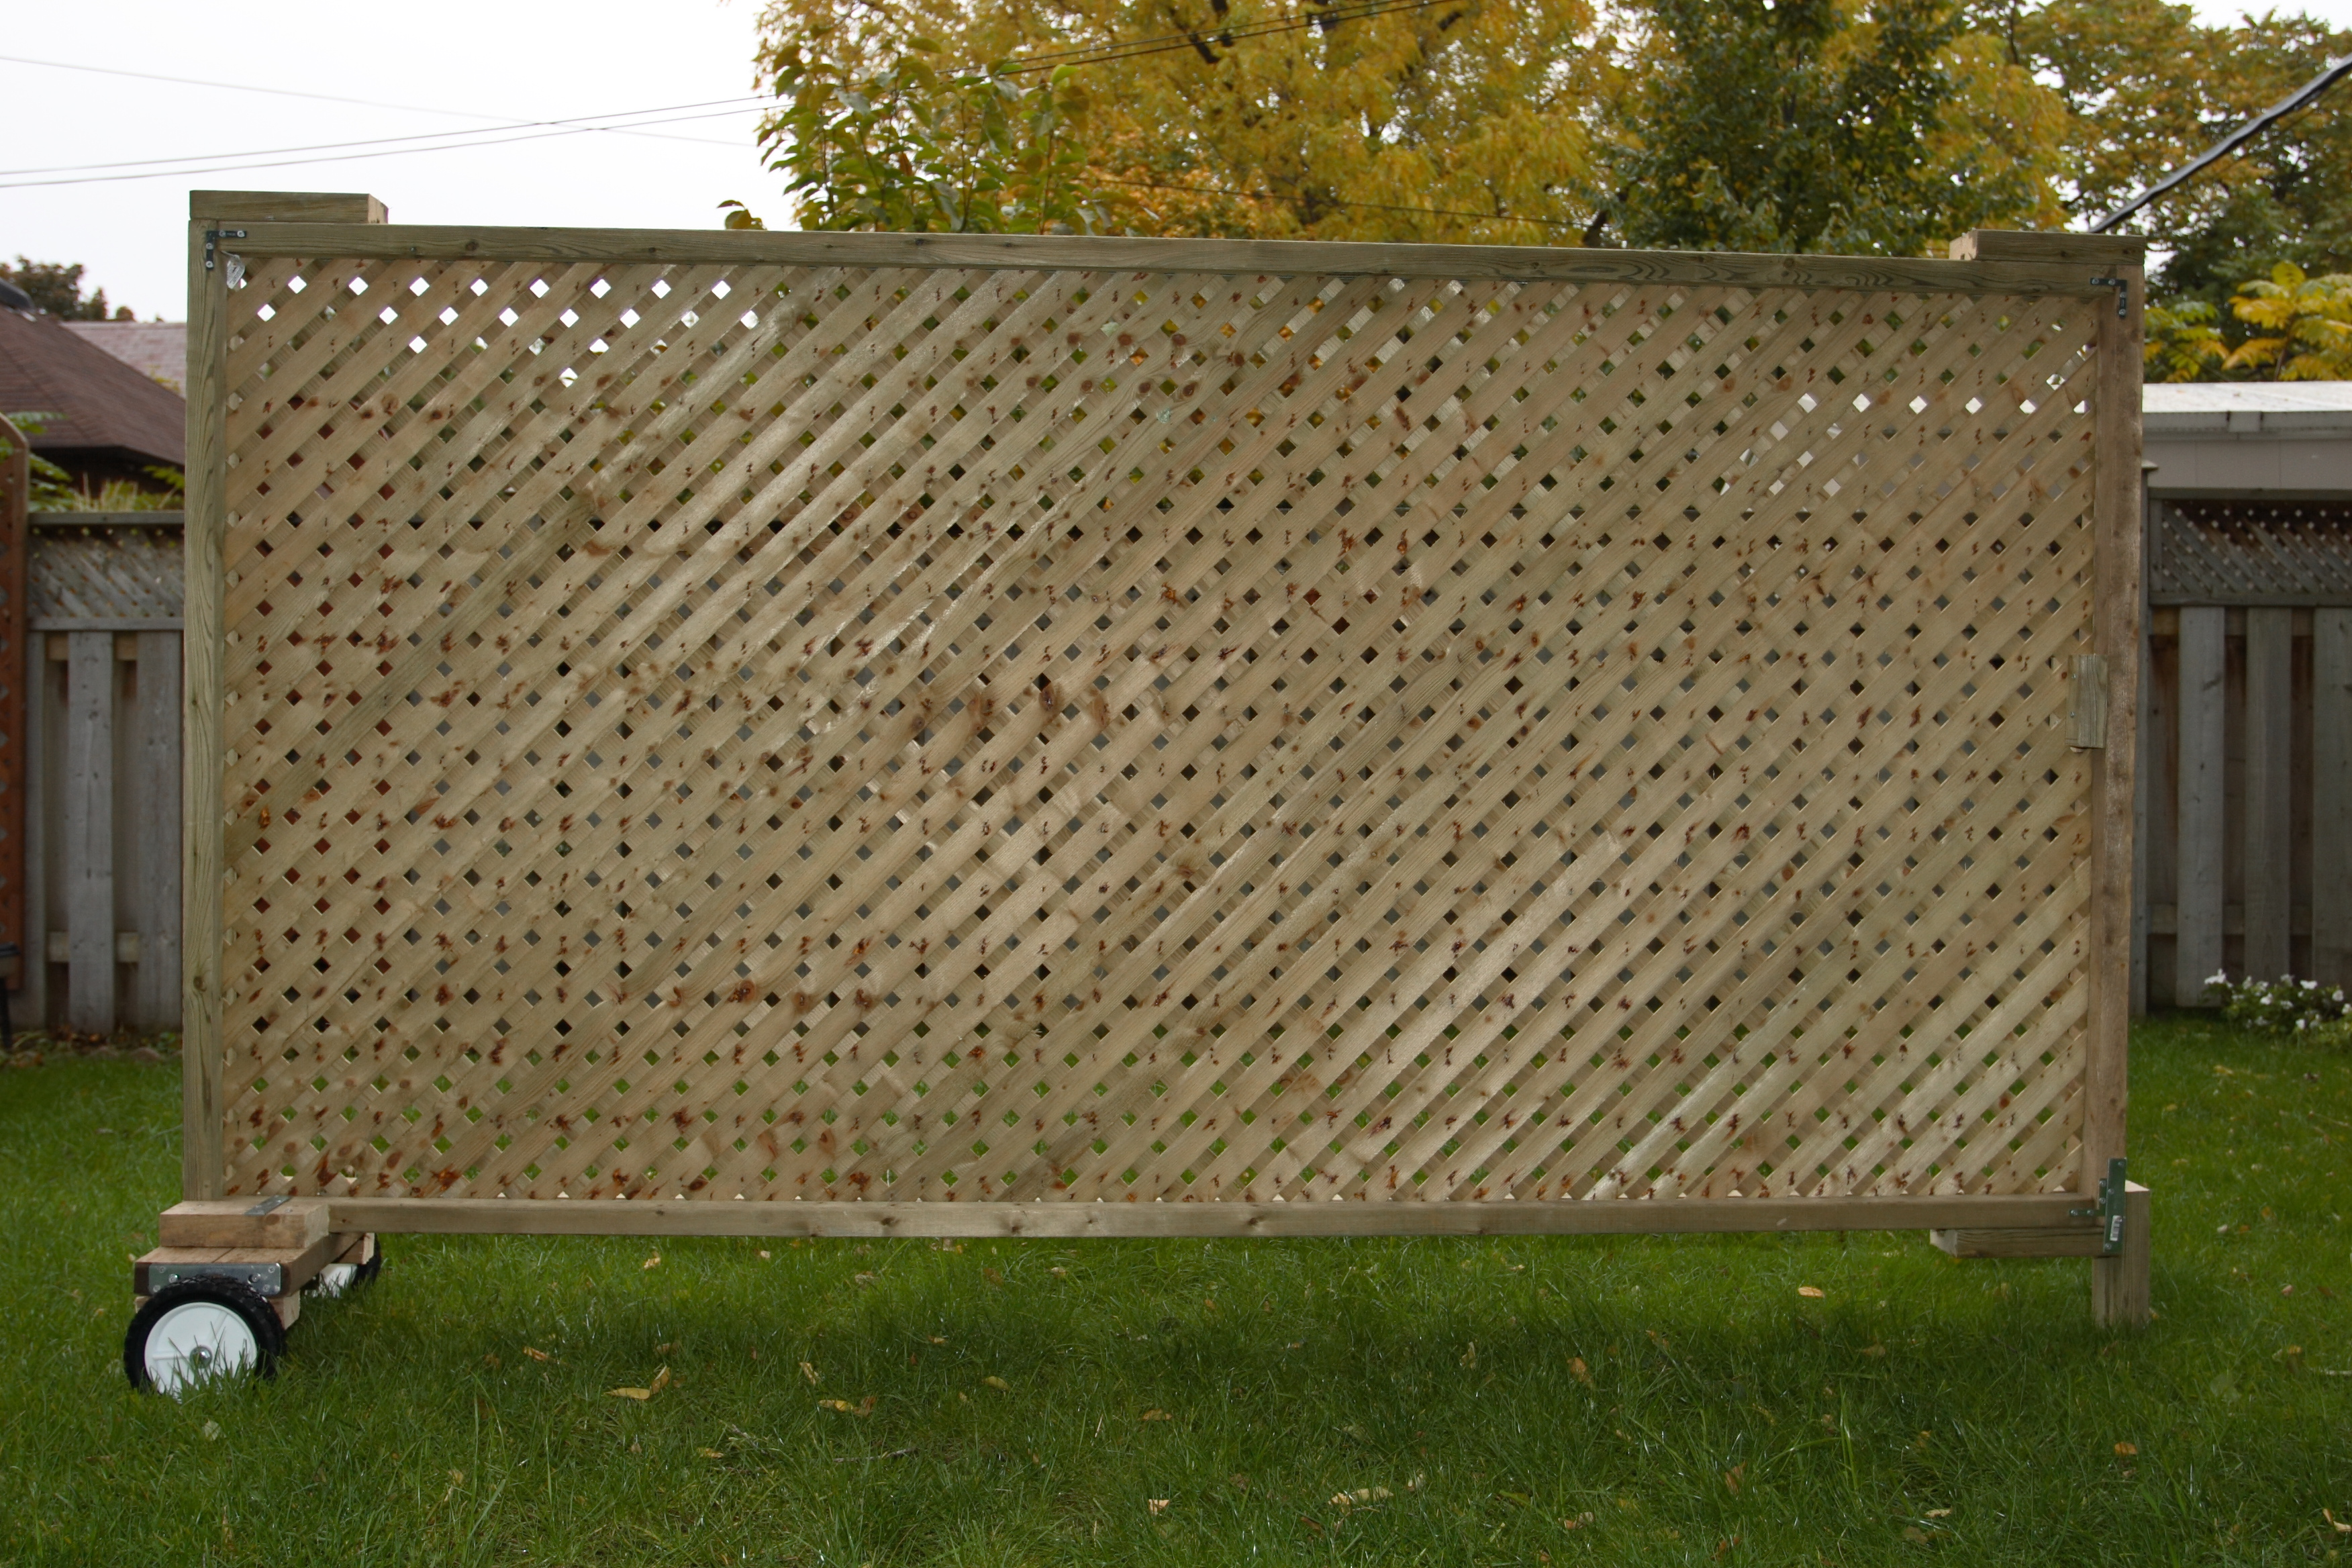
\includegraphics[scale=0.3]{screen}
\end{figure}

\end{frame}


\begin{itemize}
\item Privacy policy
\item Clear
\item Immutable
\end{itemize}


\begin{frame}[fragile]
\frametitle{Security laws}


\begin{figure}
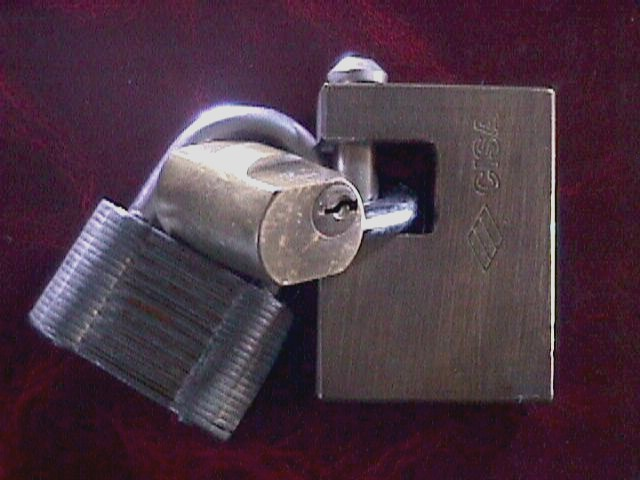
\includegraphics{security}
\end{figure}

\end{frame}


\begin{itemize}
\item Reasonable care to avoid breaches
\item Breaches must be reported
\item Delay in reporting must be signed off by law enforcement
\end{itemize}

\begin{frame}[fragile]
\frametitle{Fairness in competition laws}


\begin{figure}
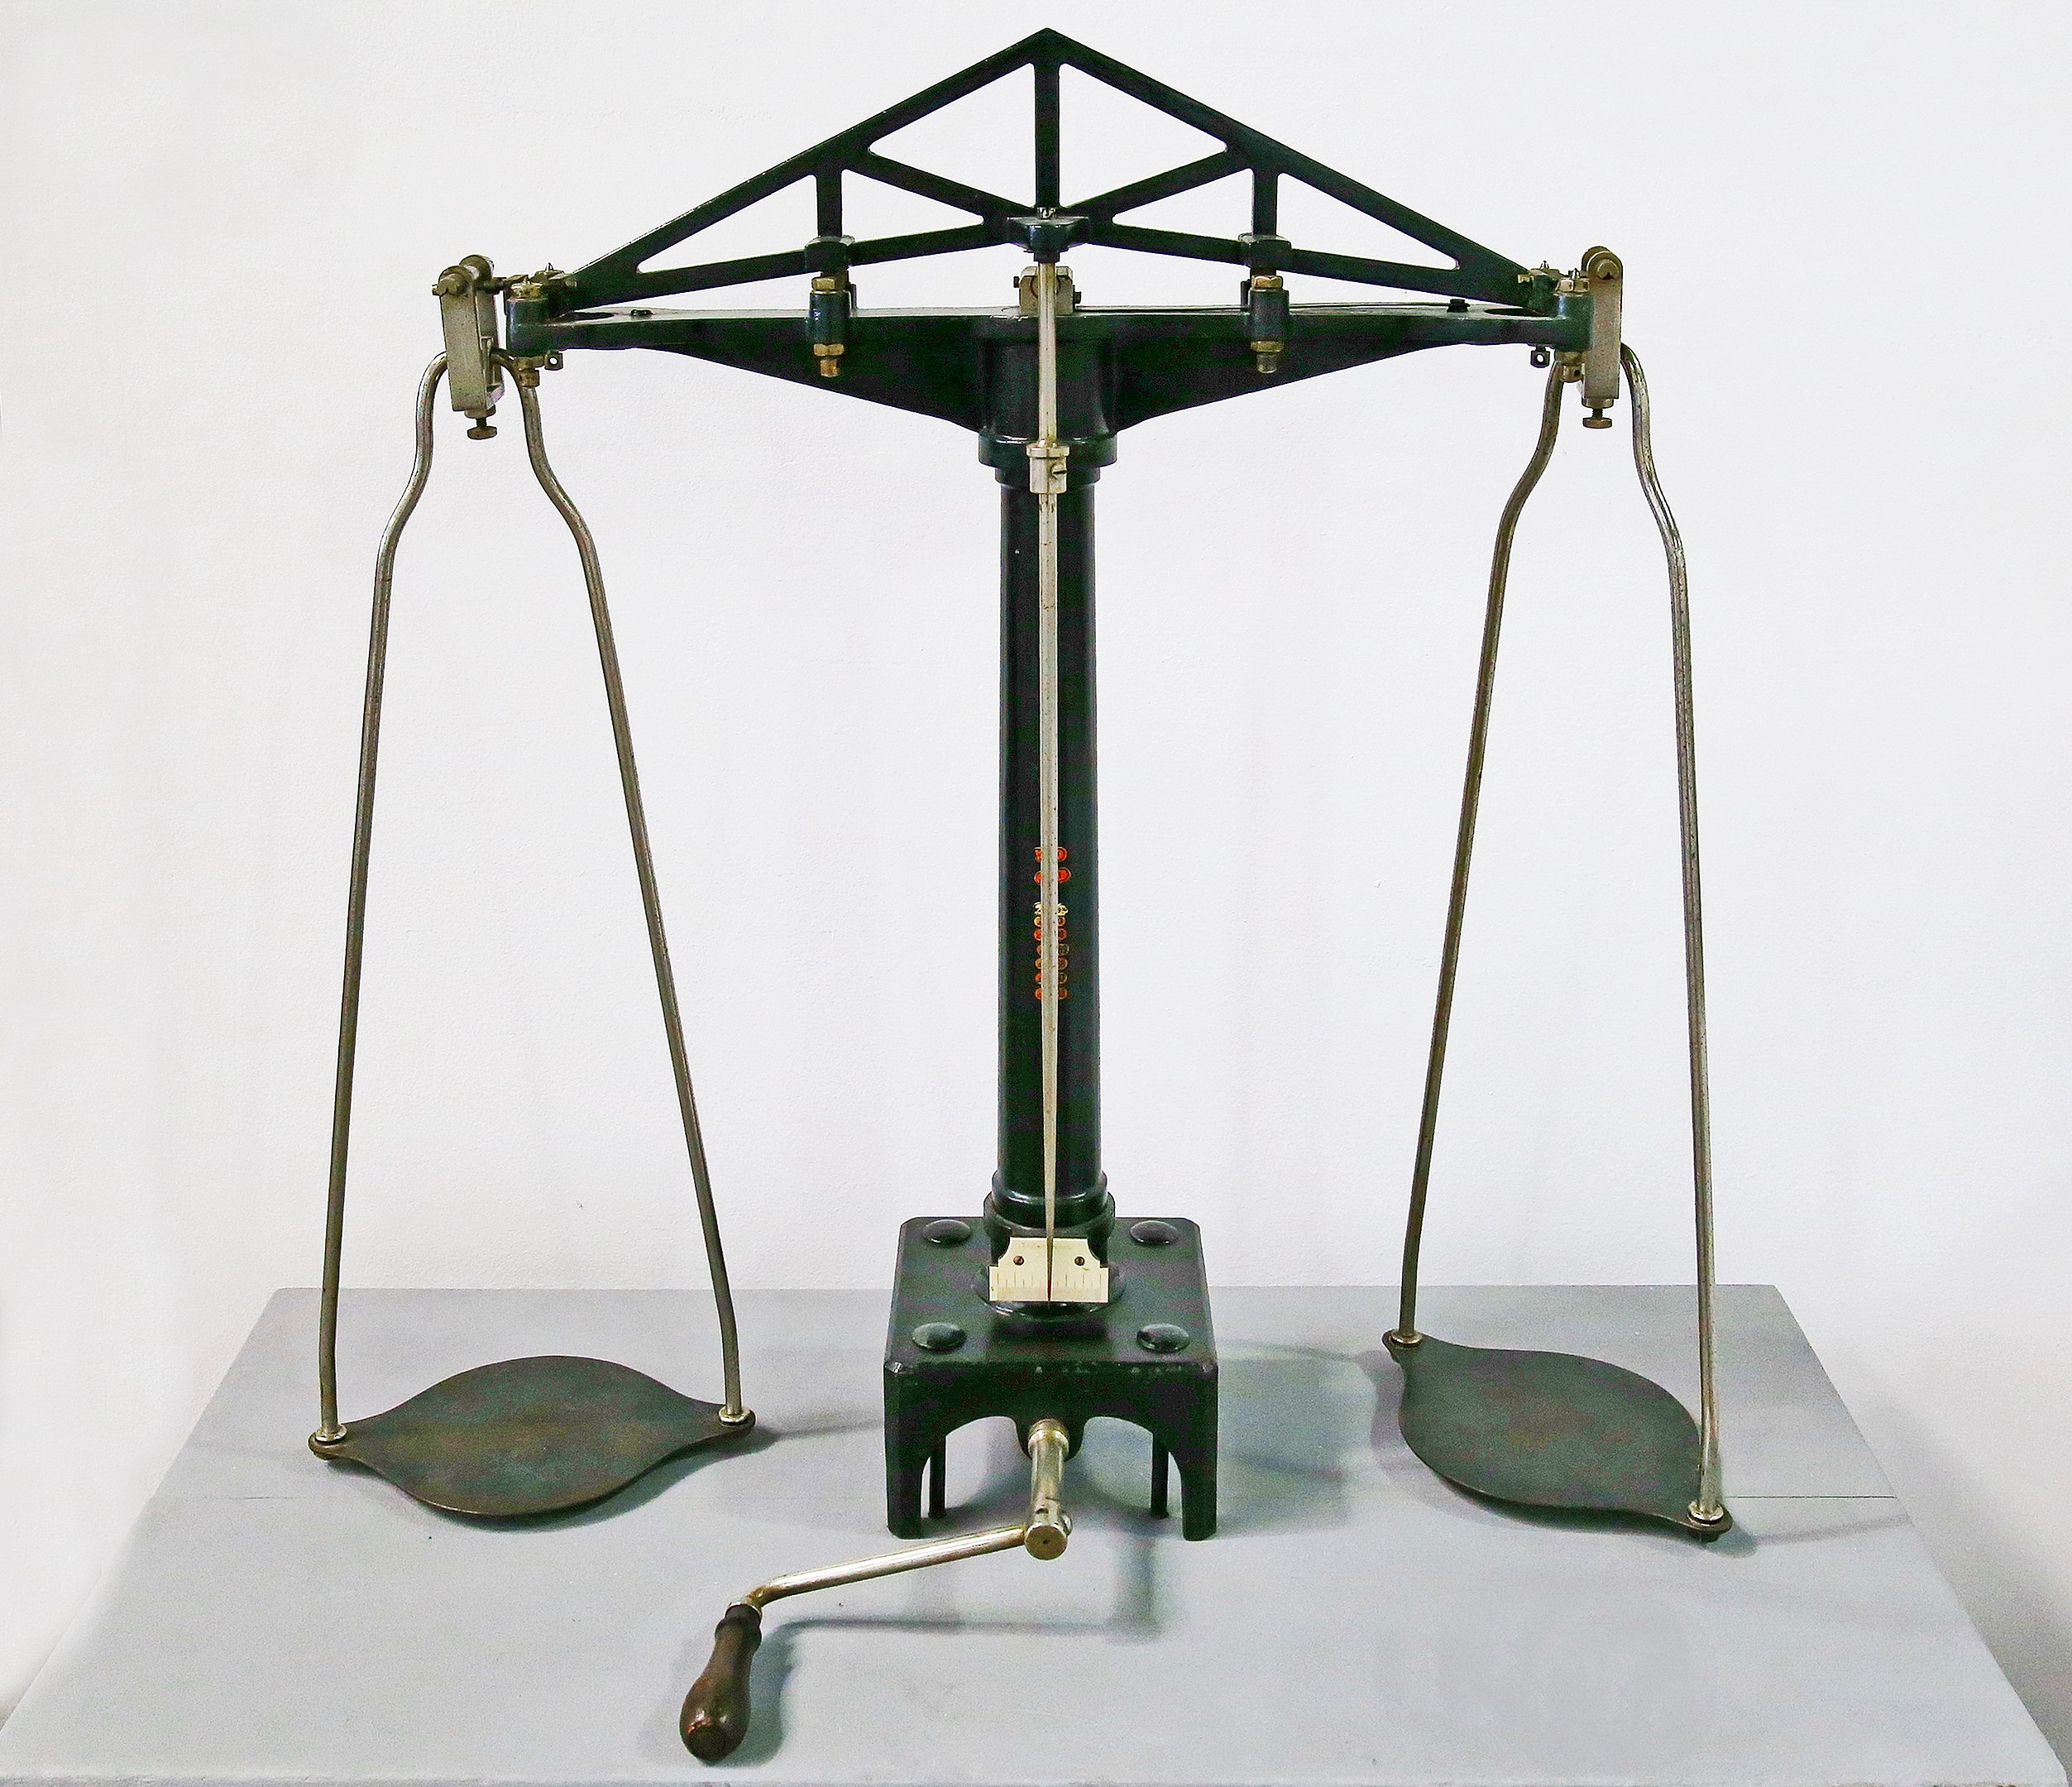
\includegraphics[scale=0.1]{scale}
\end{figure}

\end{frame}


\begin{itemize}
\item All devices must allowed all application stores
\item All web services have APIs
\item Local application data format documented
\item Only barrier to API/data access is user consent
\end{itemize}

\begin{frame}[fragile]
\frametitle{Code of Ethics}

\begin{figure}
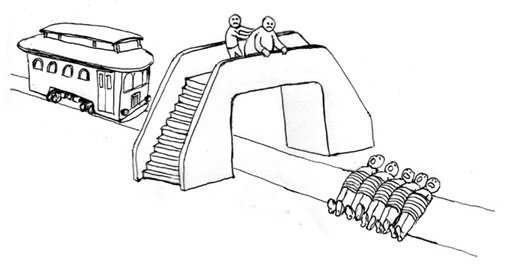
\includegraphics{fat}
\end{figure}

\end{frame}


\begin{frame}[fragile]
\frametitle{Whistelblowing}

Violations of law must be reported

\end{frame}

\begin{frame}[fragile]
\frametitle{Responsibility to principal}

Except for violations of law,
responsibility is to the development studio.

\end{frame}

\begin{frame}[fragile]
\frametitle{Commitment to competence}

Know your limits

\end{frame}

\begin{frame}[fragile]
\frametitle{Process documentation}

Document disagreements

\end{frame}

\begin{frame}[fragile]
\frametitle{Discrimination and harassment}

Beyond employment law

\end{frame}

\begin{frame}[fragile]
\frametitle{21st century: Incidents}

\begin{itemize}
\item Cambridge analytica
\item Zoom
\item Uber
\end{itemize}

\end{frame}

\begin{frame}[fragile]
\frametitle{If Not Now, When?}

Can we change the timeline?

\end{frame}


Picture credits:

\begin{itemize}
\item Picture of match: \url{https://commons.wikimedia.org/wiki/File:Streichholz.JPG}
\item Picture of fire: \url{https://commons.wikimedia.org/wiki/File:San_Francisco_Fire_Sacramento_Street_1906-04-18.jpg}
\item Picture of lock: \url{https://commons.wikimedia.org/wiki/Category:Padlocks#/media/File:Candados_2012.JPG}
\item Picture of scale: \url{https://commons.wikimedia.org/wiki/Category:Weighing_scales#/media/File:Vaga_MNT.jpg}
\item Picture of screen: \url{https://www.flickr.com/photos/garyjwood/275644014/in/photolist-qmKn1-qmKBr-oYwMG-7UWHnT-EyyT4M-qmL3a-cjf8xs-5wx88t-caR8tq-7QR7pg-6BzSc1-7U9YpL-5v4D74-6C7S53-5i8ZvA-61pcSS-5xP7Hs-5i8ZAA-caR8nd-5hygTA-5htVfK-cjhDRh-5hJXrd-au2jhs-9jX3Pw-7JaQvb-5m5PjW-5i4DBD-5m5PwE-6DPVqE-cttiCW-g5fH57-5wBrCN-6jS7DQ-ctw4mE-5hJXtC-5m5Pph-5hPBJY-6ovsi7-613SBd-6jNe5t-5m5Ptf-5iX6HH-5xRoUn-5i4DMz-5m5Prw-9nXhNt-5m1xre-caR8rh-5htVjc}
\end{itemize}

\end{document}
